\newpage
\section{Durchführung}
\label{sec:Durchführung}


\subsection{Anpassung der Schwingkreise}

Zuerst muss der anpassbare Schwingkreis an die Resonanzfrequenz des Referenzschwingkreises angepasst werden, indem dort die Kapazität variiert wird.
Also wird zunächst die Resonanzfrequenz des Referenzschwingkreises bestimmt.

\begin{figure} 
    \begin{subfigure}{0.48\textwidth}
        %\centering
        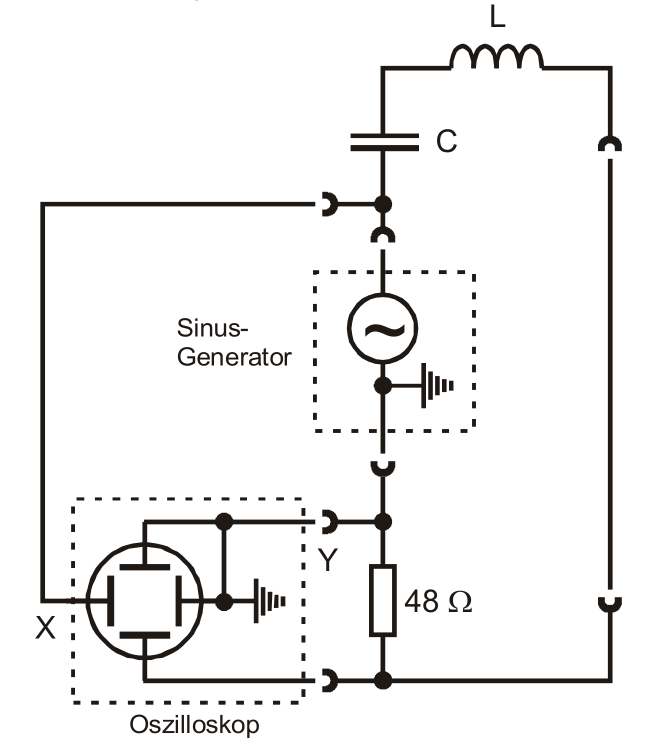
\includegraphics[height=7cm] {pictures/messschaltung.png} 
        \caption{Schematischer Aufbau. \cite{v355}}
        \label{fig:schema}
    \end{subfigure}
    \hfill
    \begin{subfigure}{0.48\textwidth}
        %\centering
        \includegraphics[height=7cm] {pictures/resonanzfrequenz.png} 
        \caption{Aufbau am Schwingkreis.}
        \label{fig:foto}
    \end{subfigure}
    \caption{Schaltung zur Bestimmung der Resonanzfrequenz.}
    \label{fig:messschaltung}
\end{figure} 

Dafür wird mithilfe der Schaltung in Abblildung \ref{fig:messschaltung} die Frequenz des Sinus-Signals solange variiert,
bis die \textit{Lissajous-Figur} die From einer Gerade annimmt. Dies kann man am  Oszilloskop visuell darstellen.
Hat man die Resonanzfrequenz gefunden, sind nun Spannung und Strom in Phase.
Hat man diese gefunden, kann man den anderen Schwingkreis passend einstellen.


\subsection{Messung}
\subsubsection*{Messung der Schwebungsfrequenz}

Nun wird die Schaltung in Abbildung \ref{fig:schwebeschaltung} mit einem Rechteckspuls angeregt.

\begin{figure} 
    \centering
    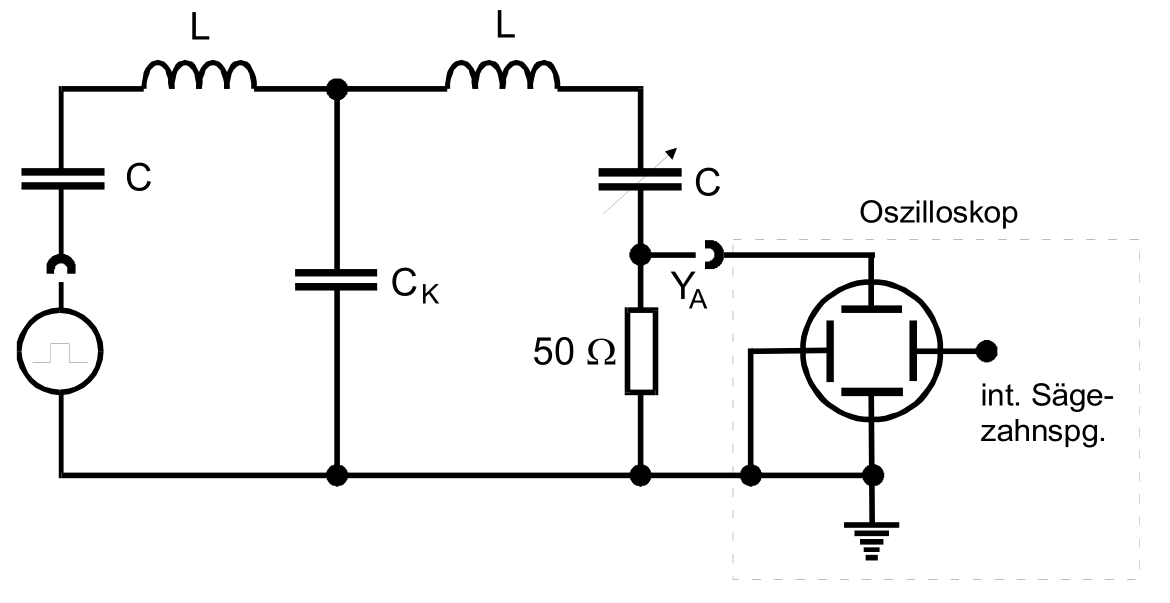
\includegraphics[width=10cm] {pictures/schwebeschaltung.png} 
    \caption{Schaltung zur Messung der Energieübertragung. \cite{v355}}
    \label{fig:schwebeschaltung}
\end{figure} 

Durch die Widerstände von $R = 48 \Omega$ wird sich ein Spannungsabfall ergeben.
Die Stromänderung wird zur Beobachtung der Schwebung am Oszilloskop visualisiert.
Jetzt werden die Maxima der Schwingung innerhalb einer Periode gezählt.

Damit lässt sich schließlich das Verhältnis der Schwebungsfrequenz und der Schwingungsfrequenz bestimmen.
Dieser Prozess wird für mehrere Kapazitäten durchgeführt.
Dabei sind Kapazitäten zwischen $C_{\text{min}} = 2 nF$ und $C_{\text{max}} = 12 nF$ möglich.


\subsubsection*{Fundamentalschwingungen}

Jetzt werden die Frequenzen $\nu^{-}$ und $\nu^{+}$ der \textit{Fundamentalschwingungen} in 
Abhängigkeit der Koppelkapazität $C_{K}$ gemessen.
Dafür wird die Anregung wieder auf eine Sinusanregung gestellt.
Zusätzlich wird die Generatorspannung als x-Ablenkung benutzt.
Nun sucht man wie zu Beginn mithilfe der Lissajous-Figuren die Frequenzen, bei denen die Phase 0 oder $\pi$ ist.
Dies wird für alle kapazitäten $C_{k}$ durchgeführt.


\subsubsection*{Verlauf der Ströme}

Im Folgenden werden die Verläufe der Ströme $I_{K}$ und $I_{2}$ in Abhängigkeit von der Frequenz
mithilfe der Schaltung in Abbildung \ref{fig:stromkurven} untersucht.

\begin{figure} 
    \centering
    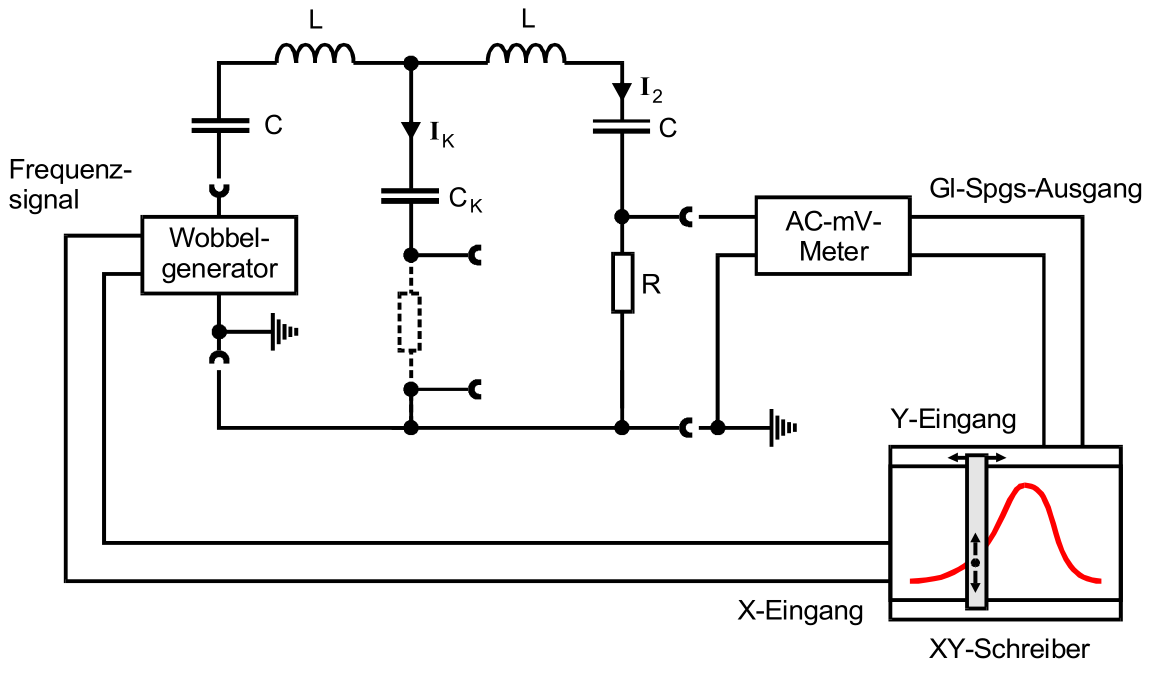
\includegraphics[width=10cm] {pictures/stromkurven.png} 
    \caption{Schaltung zur Aufnahme der Stromkurven. \cite{v355}}
    \label{fig:stromkurven}
\end{figure} 

Dafür wird der Spannungsabfall in den Widerständen mit einem AC-Breitband-Millivoltmeter gemessen.
Der sogenannte \textit{Wobbelgenerator} gibt neben der Wechselspannung auch noch ein Gleichspannungssignal.
Mit diesen Spannung lässt sich der XY-Schreiber ansteuern und  den Strom in Abhängigkeit der Frequenz visualisiert.
